\section{Introduction}
\IEEEPARstart{I}{ndustrial} agent integration couples online data acquisition with governed control. The agent gathers process observations and production context, weighs them against an objective, and proposes a typed setpoint or recipe adjustment. Before any write, the runtime resolves which line, process variable, and control signal the request concerns, then applies authority and limits. In practice, a cast-film line-speed setpoint may affect measured film thickness, yet the control and acquisition nodes remain distinct even when both use Message Queuing Telemetry Transport (MQTT). Acquired observations, command acceptance, device readback, and later process measurements are therefore separate evidence, as Fig.~\ref{fig:control-path} illustrates.

Prior work on industrial agents addresses service supervision and skill-based manufacturing~\cite{biskupovic2025supervision,koehle2026llmdriven}, semantic grounding and verification for plant-facing operations including programmable logic controller (PLC) interfaces~\cite{graul2026aas,schall2026safe}, and multi-agent fault-recovery planning~\cite{vyas2026detection}. These strands establish relevant capabilities but leave an integration question: how can online acquisition and analysis connect to governed operations across task-mediated and direct entry paths? This paper examines that runtime boundary; it introduces no new control law or agent-reasoning algorithm.

Five invariants govern the design: (i) observations may inform an agent's proposal but never grant write authority; (ii) acquisition and control mappings are direction-specific; (iii) an approved control intent is revalidated before dispatch; (iv) command receipts, readbacks, and later process observations remain separate records, and task-mediated and direct calls converge on one guarded boundary; and (v) a scene binds line, product, recipe, and run to mappings, drivers, objectives, and limits.

The contributions are:
\begin{enumerate}
  \item A production-scene model that links context, direction-specific acquisition and control mappings, registered drivers, objectives, and limits into one agent-facing operation contract. (Section~III.)
  \item An agent-to-operation boundary in which registered agent harnesses (adapters that expose the runtime's scoped tools to a model) acquire observations and submit control intents, while task-mediated and direct calls share one dispatcher and the applicable route-specific approval, revalidation, and write guards. (Sections~III--V.)
  \item An evidence-bounded evaluation of these mappings and governance responses, together with an exploratory simulator comparison and language-model-driven episodes. (Section~VI.)
\end{enumerate}

\begin{figure}[!b]
\centering
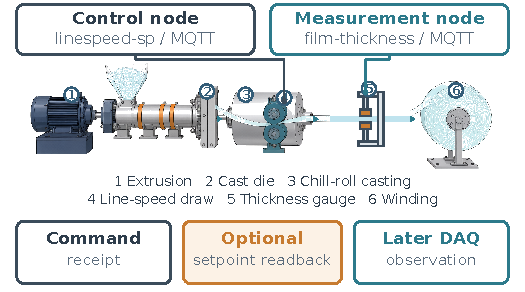
\includegraphics[width=0.98\columnwidth]{resources/fig1-vectorized-20261109.pdf}
\caption{Cast-film flow: extrusion (1), cast die (2), chill-roll casting (3), line-speed draw (4), thickness gauging (5), winding (6). The \texttt{linespeed-sp} control and \texttt{film-thickness} acquisition nodes stay distinct despite sharing MQTT; leaders mark draw rolls and gauge. Writes yield command receipts and optional readbacks; later thickness values are separate data-acquisition (DAQ) observations.}
\label{fig:control-path}
\end{figure}


